\section{Piecewise Linear Interpolation}
\label{example:PiecewiseLinearInterpolcation}

The piecewise linear interpolation is an extension of the linear interpolation for two data points discussed in Example \ref{example:LinearInterpolcation}. It can be used to approximate any polynomial functions. Graphically,

\begin{figure}[h]
\centering
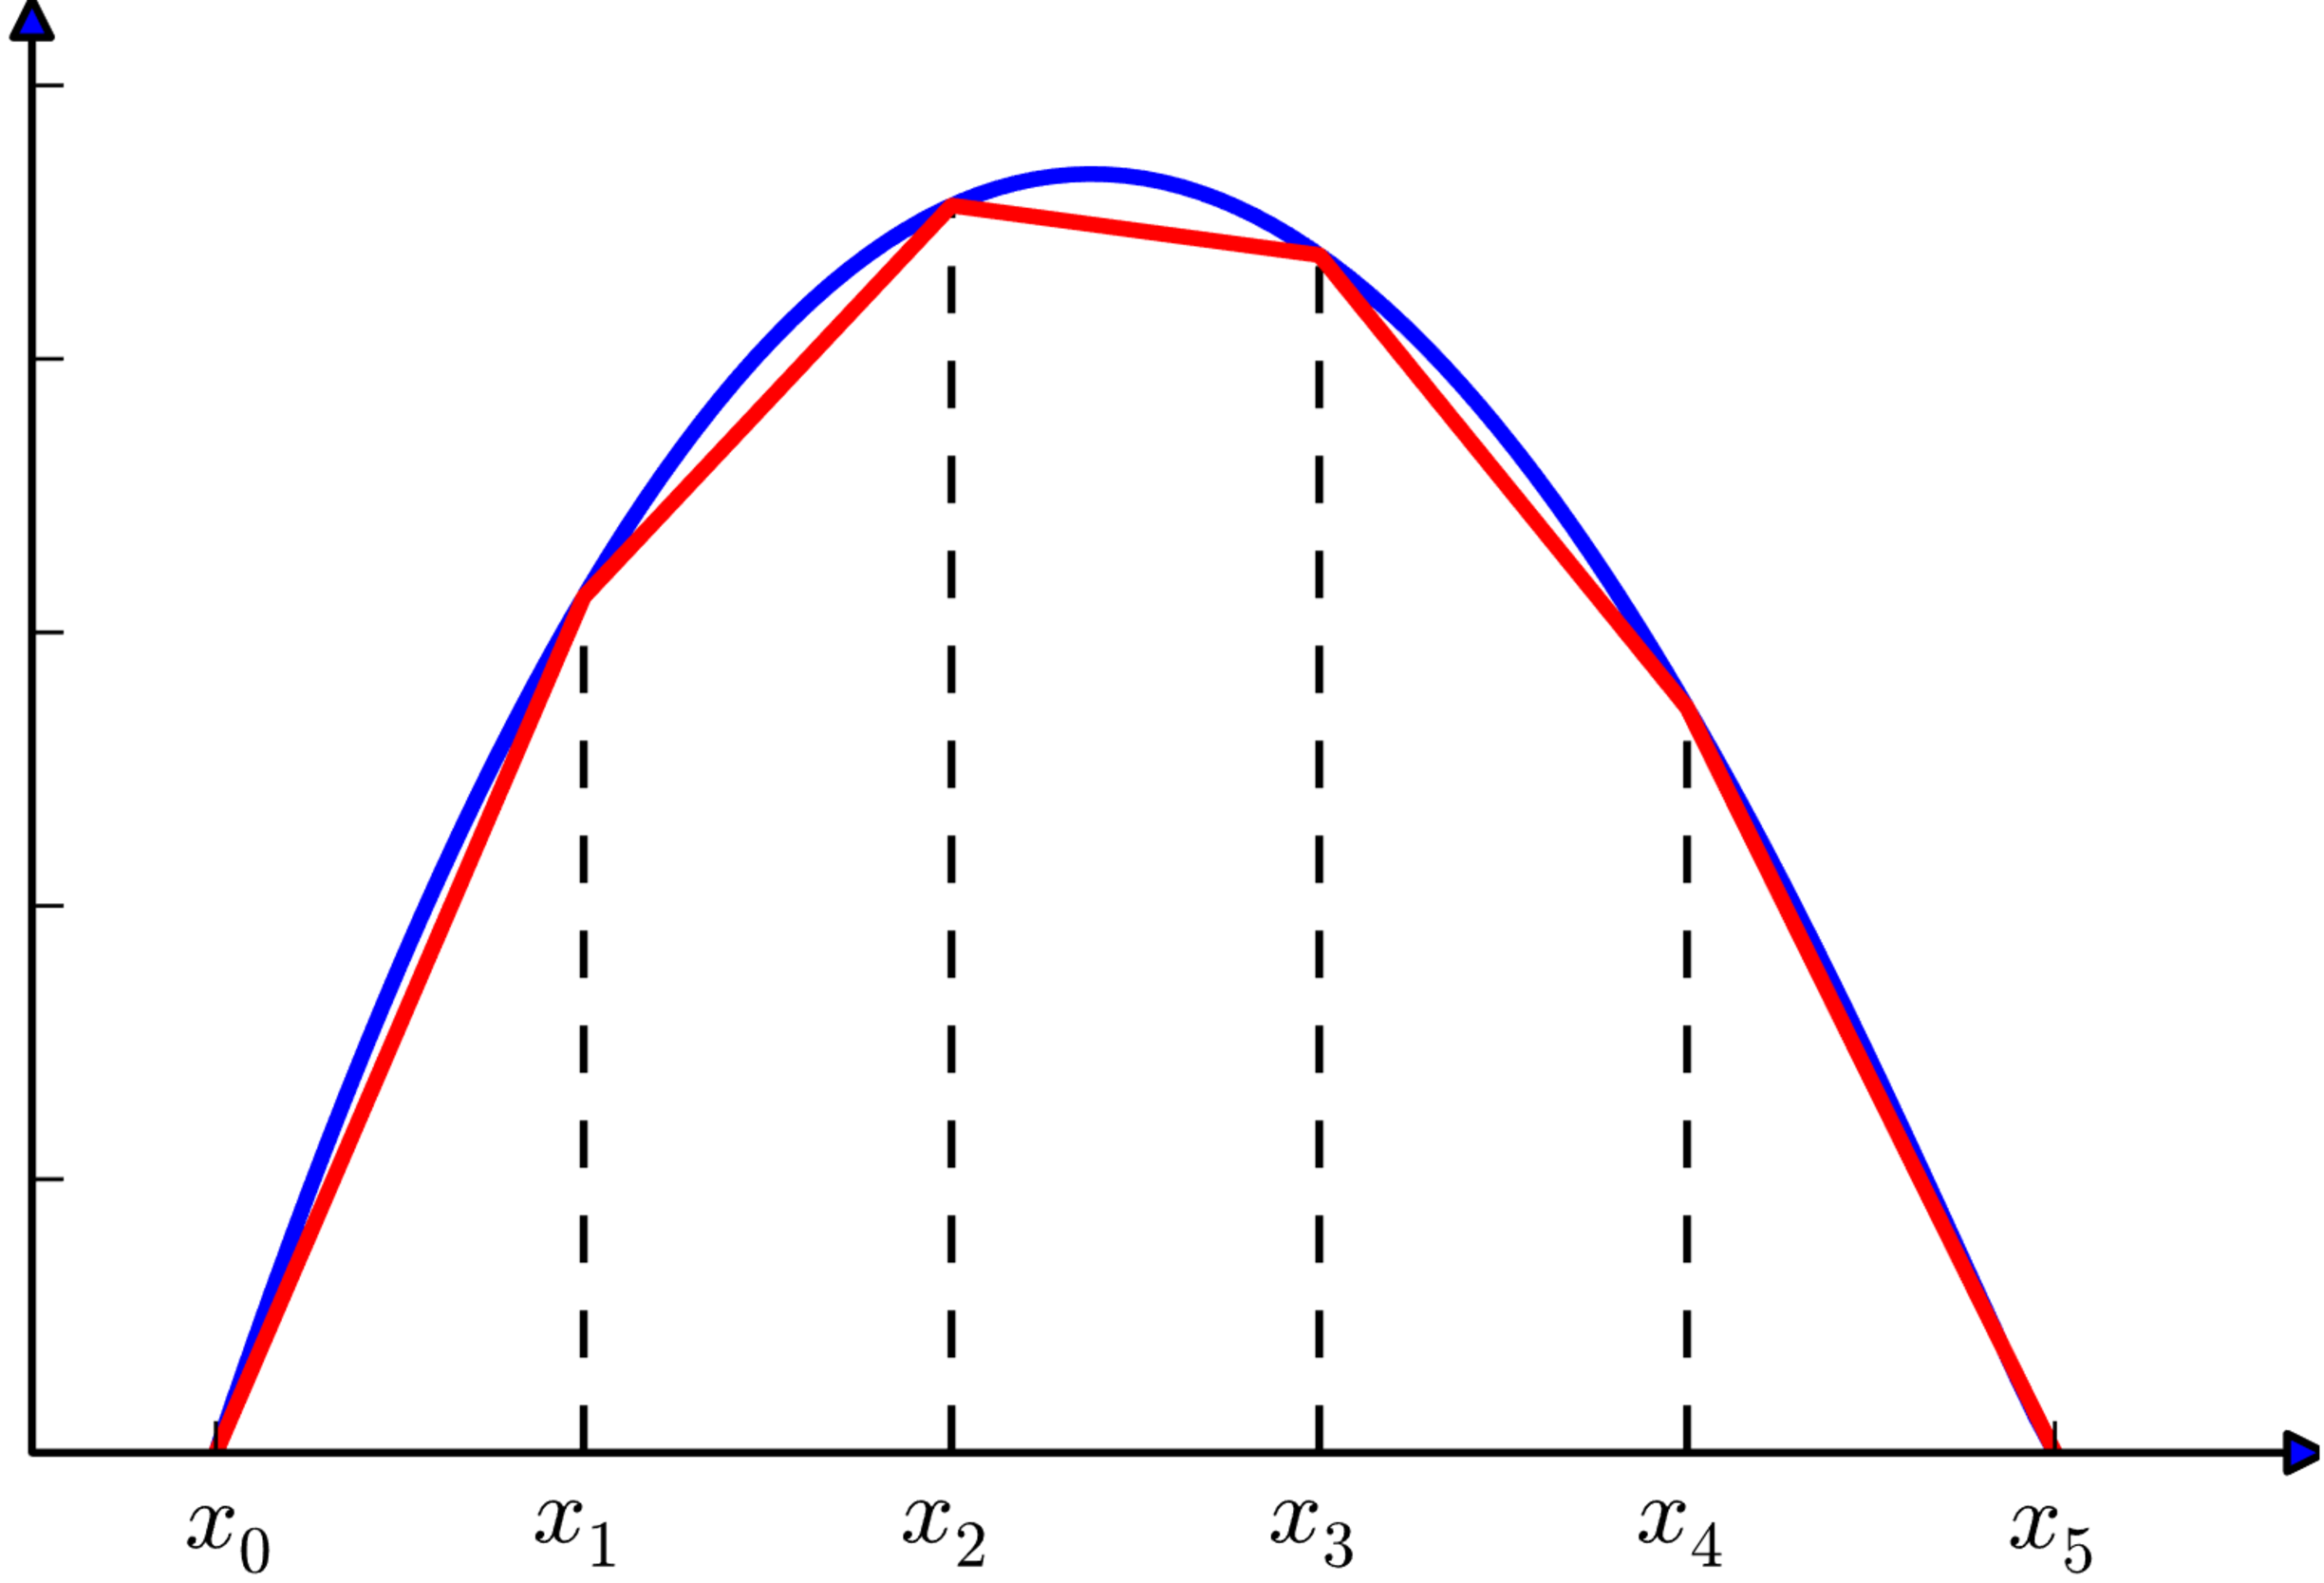
\includegraphics[width=10cm]{./figures/PiecewiseLinear.pdf}
\caption{Piecewise linear}
\label{fig:PiecewiseLinear}
\end{figure}

Suppose that we have $n$ data points: $(x_1, y_1), (x_2, y_2), \cdots, (x_i, y_i), \cdots (x_n, y_n)$ and the $x$-coordinate of the interpolation point is $z$. The piecewise linear interpolant is built upon the local linear interpolants.

$$
L(z) = 
\begin{cases}
\enspace L_1(z) & \text{ if } x_1 \le z < x_2, \\
\enspace L_2(z) & \text{ if } x_2 \le z < x_3, \\
\enspace \quad\vdots & \qquad\quad\vdots \\
\enspace L_i(z) & \text{ if } x_i \le z < x_{i+1}, \\
\enspace \quad\vdots & \qquad\quad\vdots \\
\enspace L_{n-1}(z) & \text{ if } x_{n-1} \le z < x_n,
\end{cases}
$$

where

$$
L_i(z) = \left(1-\frac{z-x_i}{x_{i+1}-x_i}\right) \cdot y_i + \frac{z-x_i}{x_{i+1}-x_i} \cdot y_{i+1}
$$

So once we find the interval $[x_i, x_{i+1})$ where the interpolation point falls into, we can simply call the function defined in Example \ref{example:LinearInterpolcation} to compute the interpolated value.

\subsection{Implementation}
The function belows takes three arguments with $n \ge 2$:

\begin{itemize}
\item \q{x} - a list of $x$-coordinates, \emph{i.e.} $x = (x_1, x_2, \cdots, x_i, \cdots, x_n)$
\item \q{y} - a list of $y$-coordinates, \emph{i.e.} $y = (y_1, y_2, \cdots, y_i, \cdots, y_n)$
\item \q{z} - the $x$-coordinate of the interpolation point
\end{itemize}

So there are $n$ data points in the above example and $(x_i,y_i)$ is the data point $i$.

\begin{minted}[samepage,frame=single,framesep=10pt,xleftmargin=10pt,linenos]{q}
.qe.math.pwlerp:{[x;y;z]
  if[all x=asc x;'"First argument must be in ascending order"];
  if[z>=last x;:last y];
  if[z<=first x;:first y];
  i:bin[`float$x;`float$z];
  x:@[x;(i;i+1)];
  y:@[y;(i;i+1)];
  .qe.math.lerp[x;y;z]
  };
\end{minted}


\subsection{Explanations}
In the implementation above,

\begin{itemize}
\item Line 2 checks whether the first argument is in ascending order. Otherwise, an error is thrown.
\item Line 3 checks whether the $x$-coordinate of the interpolation point is greater the largest $x$-coordinate of all data points. If so, return the $y$-coordinate of the last data point.
\item Line 4 checks whether the $x$-coordinate of the interpolation point is smaller the smallest $x$-coordinate of all data points. If so, return the $y$-coordinate of the first data point.
\item Line 5 finds the index of the interval where the interpolation point falls into. We also convert the two arguments of \q{bin} to \q{float} type to avoid potential \q{type} error.
\item Lines 6 and 7 narrow down the endpoints for the local interpolant.
\item Line 8 calls the linear interpolation function defined earlier.
\end{itemize}


\subsection{Summary}

\begin{importantblock}
\textbf{Important Note}
\begin{itemize}
\item The argument \q{x} must be in ascending order in this implementation.
\end{itemize}
\end{importantblock}

\begin{noteblock}
\textbf{Knowledge Points}
\begin{itemize}
\item Functions \href{https://code.kx.com/q/ref/if/}{\q{if}}, \href{https://code.kx.com/q/ref/all-any/#all}{\q{all}}, \href{https://code.kx.com/q/ref/asc/}{\q{asc}}, \href{https://code.kx.com/q/ref/first/#first}{\q{first}} and \href{https://code.kx.com/q/ref/first/#last}{\q{last}} 
\item Type casting: \href{https://code.kx.com/q/ref/cast/}{\q{$}}
\item Error signalling: \href{https://code.kx.com/q/ref/signal/}{\q{'}}
\item Binary search: \href{https://code.kx.com/q/ref/bin/}{\q{bin}}
\item Apply at index: \href{https://code.kx.com/q/ref/apply/#apply-at-index-at}{\q{@}}
\end{itemize}
\end{noteblock}


\clearpage
